\subsection{Examples}

\begin{concept}{Subroutine Basics}\\
Key components of subroutines:
\begin{itemize}
  \item \textbf{Calling Convention}:
    \begin{itemize}
      \item Parameters passed in R0-R3
      \item Return value in R0
      \item Link Register (LR) for return address
      \item Stack for additional parameters/locals
    \end{itemize}
  \item \textbf{Register Usage}:
    \begin{itemize}
      \item R0-R3: Parameters and scratch
      \item R4-R11: Must be preserved
      \item R12: IP (scratch)
      \item R13: SP (stack pointer)
      \item R14: LR (link register)
      \item R15: PC (program counter)
    \end{itemize}
\end{itemize}
\end{concept}

\begin{example2}{Nested Subroutine Calls}\\
Example of multiple nested calls with stack manipulation:
\begin{lstlisting}[language=armasm, style=basesmol]
    AREA    progCode, CODE, READONLY
    THUMB
main
    LDR     R1, =0x10203040     ; Initial values
    LDR     R2, =0x50607080
    BL      procA               ; Call procA
    BL      procB               ; Call procB
    B       endless

procA
    PUSH    {R1, R2}            ; Save registers
    LDR     R1, =0xAABBCCDD     ; New values
    LDR     R2, =0xEEFF1020
    POP     {R1, R2}            ; Restore registers
    BX      LR                  ; Return

procB
    PUSH    {R1, R2, LR}        ; Save including LR
    LDR     R1, =0x11223344     ; New values
    LDR     R2, =0x55667788
    BL      procC               ; Call procC
    POP     {R1, R2, PC}        ; Return by popping PC

procC
    PUSH    {R1, R2, LR}        ; Save registers
    LDR     R1, =0x11111111     ; New values
    LDR     R2, =0x22222222
    BL      procD               ; Call procD
    POP     {R1, R2, PC}        ; Return by popping PC
\end{lstlisting}

Stack contents at key points:
\begin{itemize}
  \item After procA PUSH: R1(0x10203040), R2(0x50607080)
  \item After procB PUSH: R1, R2, LR(ret\_addr)
  \item After procC PUSH: R1(0x11223344), R2(0x55667788), LR(ret\_addr)
\end{itemize}
\end{example2}

\begin{KR}{Subroutine Implementation}\\
Guidelines for implementing subroutines:

1. Basic subroutine:
\begin{lstlisting}[language=armasm, style=basesmol]
proc_name
    PUSH    {LR}           ; Save return address
    ; Subroutine code
    POP     {PC}           ; Return
\end{lstlisting}

2. With register preservation:
\begin{lstlisting}[language=armasm, style=basesmol]
proc_name
    PUSH    {R4-R7, LR}    ; Save modified registers
    ; Subroutine code using R4-R7
    POP     {R4-R7, PC}    ; Restore and return
\end{lstlisting}

3. With local variables:
\begin{lstlisting}[language=armasm, style=basesmol]
proc_name
    PUSH    {R4, LR}       ; Save registers
    SUB     SP, SP, #8     ; Allocate locals
    ; Use [SP] to [SP, #4] for locals
    ADD     SP, SP, #8     ; Deallocate locals
    POP     {R4, PC}       ; Restore and return
\end{lstlisting}
\end{KR}

\begin{example2}{Stack Frame Management}\\
Example showing stack frame creation and cleanup:

\begin{lstlisting}[language=armasm, style=basesmol]
func    ; Function prologue
    PUSH    {R4-R8, LR}    ; Save registers
    SUB     SP, SP, #12    ; Allocate locals
    
    ; Access local variables relative to SP
    STR     R0, [SP, #0]   ; Local var 1
    STR     R1, [SP, #4]   ; Local var 2
    STR     R2, [SP, #8]   ; Local var 3
    
    ; Function body
    BL      other_func     ; Call another function
    
    ; Function epilogue
    ADD     SP, SP, #12    ; Deallocate locals
    POP     {R4-R8, PC}    ; Restore and return
\end{lstlisting}
\end{example2}

\begin{concept}{Stack Operations}\\
Common stack manipulation patterns:
\begin{itemize}
  \item \textbf{Register Save/Restore}:
    \begin{itemize}
      \item PUSH/POP for callee-saved registers
      \item Multiple register transfer
    \end{itemize}
  \item \textbf{Local Variables}:
    \begin{itemize}
      \item SUB SP to allocate space
      \item Access via SP-relative addressing
      \item ADD SP to deallocate space
    \end{itemize}
  \item \textbf{Return Handling}:
    \begin{itemize}
      \item Save LR if making calls
      \item Return via BX LR or POP \{PC\}
      \item Use PC in POP list when LR saved
    \end{itemize}
\end{itemize}
\end{concept}

\begin{KR}{Stack Frame Layout}\\
Guidelines for managing stack frames:

1. Frame structure:
\begin{itemize}
  \item Previous stack frame
  \item Return address (LR)
  \item Saved registers
  \item Local variables
  \item Parameters for called functions
\end{itemize}

2. Frame creation:
\begin{lstlisting}[language=armasm, style=basesmol]
    ; Save registers and create frame
    PUSH    {R4-R7, LR}    ; Save registers
    SUB     SP, SP, #frame_size  ; Allocate space
    
    ; Initialize frame if needed
    MOV     R4, #0         ; Clear locals
    STR     R4, [SP, #0]   ; Initialize var1
    STR     R4, [SP, #4]   ; Initialize var2
\end{lstlisting}

3. Frame access:
\begin{lstlisting}[language=armasm, style=basesmol]
    ; Access local variables
    LDR     R0, [SP, #offset1]  ; Load local1
    STR     R1, [SP, #offset2]  ; Store to local2
    
    ; Access parameters beyond R0-R3
    LDR     R0, [SP, #param_offset] ; Load param
\end{lstlisting}

4. Frame cleanup:
\begin{lstlisting}[language=armasm, style=basesmol]
    ; Deallocate frame and restore
    ADD     SP, SP, #frame_size  ; Remove locals
    POP     {R4-R7, PC}    ; Restore and return
\end{lstlisting}
\end{KR}

\begin{remark}
Important considerations:
\begin{itemize}
  \item Maintain 8-byte stack alignment
  \item Save LR before any BL instructions
  \item Properly pair PUSH/POP operations
  \item Document stack frame layout
  \item Track stack depth in nested calls
\end{itemize}
\end{remark}

\section*{CT1 Übungsaufgaben}
\section*{Unterprogramme und Stack}
\section*{Aufgabe}
Im folgenden Assembler-Programm werden die vier Unterprogramme procA, procB, procC und procD aufgerufen und einige Register mit PUSH gesichert und zurückgeladen. Zu Beginn des Programmes steht der Stackpointer (SP) auf 0x20000660.\\
Bestimmen Sie zu den angegebenen Zeitpunkten Z1. . . Z4 den Inhalt des Stacks. Schreiben Sie daneben die Bedeutung des Stack-Inhaltes, z.B. Inhalt R1 von procX oder ret adr von procY).

\begin{center}
\begin{tabular}{|c|c|c|c|}
\hline
28 & endless &  &  \\
\hline
29 0x0800079C 490D & LDR & $\mathrm{R} 1,=0 \times 10203040$ &  \\
\hline
$300 \times 0800079 \mathrm{4}$ 40E & LDR & $\mathrm{R} 2,=0 \times 50607080$ &  \\
\hline
31 0x080007A0 F000 F804 & BL & procA &  \\
\hline
32 0x080007A4 F000 F807 & BL & procB &  \\
\hline
33 0x080007A8 E7F8 & B & endless &  \\
\hline
$340 \times 080007 A A 0000$ & ALIGN &  &  \\
\hline
39 & procA &  &  \\
\hline
40 0x080007AC B406 & PUSH & \{R1, R2\} &  \\
\hline
41 &  &  & ; <------------- (Z1) \\
\hline
42 0x080007AE 490B & LDR & R1, =0xAABBCCDD &  \\
\hline
43 0x080007B0 4A0B & LDR & R2, =0xEEFF1020 &  \\
\hline
44 0x080007B2 BC06 & POP & \{R1, R2\} &  \\
\hline
45 0x080007B4 4770 & BX & LR &  \\
\hline
46 &  &  &  \\
\hline
47 & procB &  &  \\
\hline
48 0x080007B6 B506 & PUSH & \{R1, R2, LR \} &  \\
\hline
49 &  &  & ; <------------- (Z2) \\
\hline
50 0x080007B8 490A & LDR & R1, $=0 \times 11223344$ &  \\
\hline
51 0x080007BA 4A0B & LDR & R2, $=0 \times 55667788$ &  \\
\hline
52 0x080007BC F000 F801 & BL & procC &  \\
\hline
53 0x080007C0 BD06 & POP & \{R1, R2, PC\} &  \\
\hline
54 &  &  &  \\
\hline
55 & procC &  &  \\
\hline
56 0x080007C2 B506 & PUSH & \{R1, R2, LR \} &  \\
\hline
57 &  &  & ; <------------- (Z3) \\
\hline
$580 \times 080007 \mathrm{C} 44909$ & LDR & R1, $=0 \times 11111111$ &  \\
\hline
59 0x080007C4 4A0A & LDR & $\mathrm{R} 2,=0 \times 2222222$ &  \\
\hline
60 0x080007C8 F000F801 & BL & procD &  \\
\hline
61 0x080007CC BD06 & POP & \{R1, R2, PC \} &  \\
\hline
62 &  &  & ; <------------- (Z4) \\
\hline
\end{tabular}
\end{center}

\begin{center}
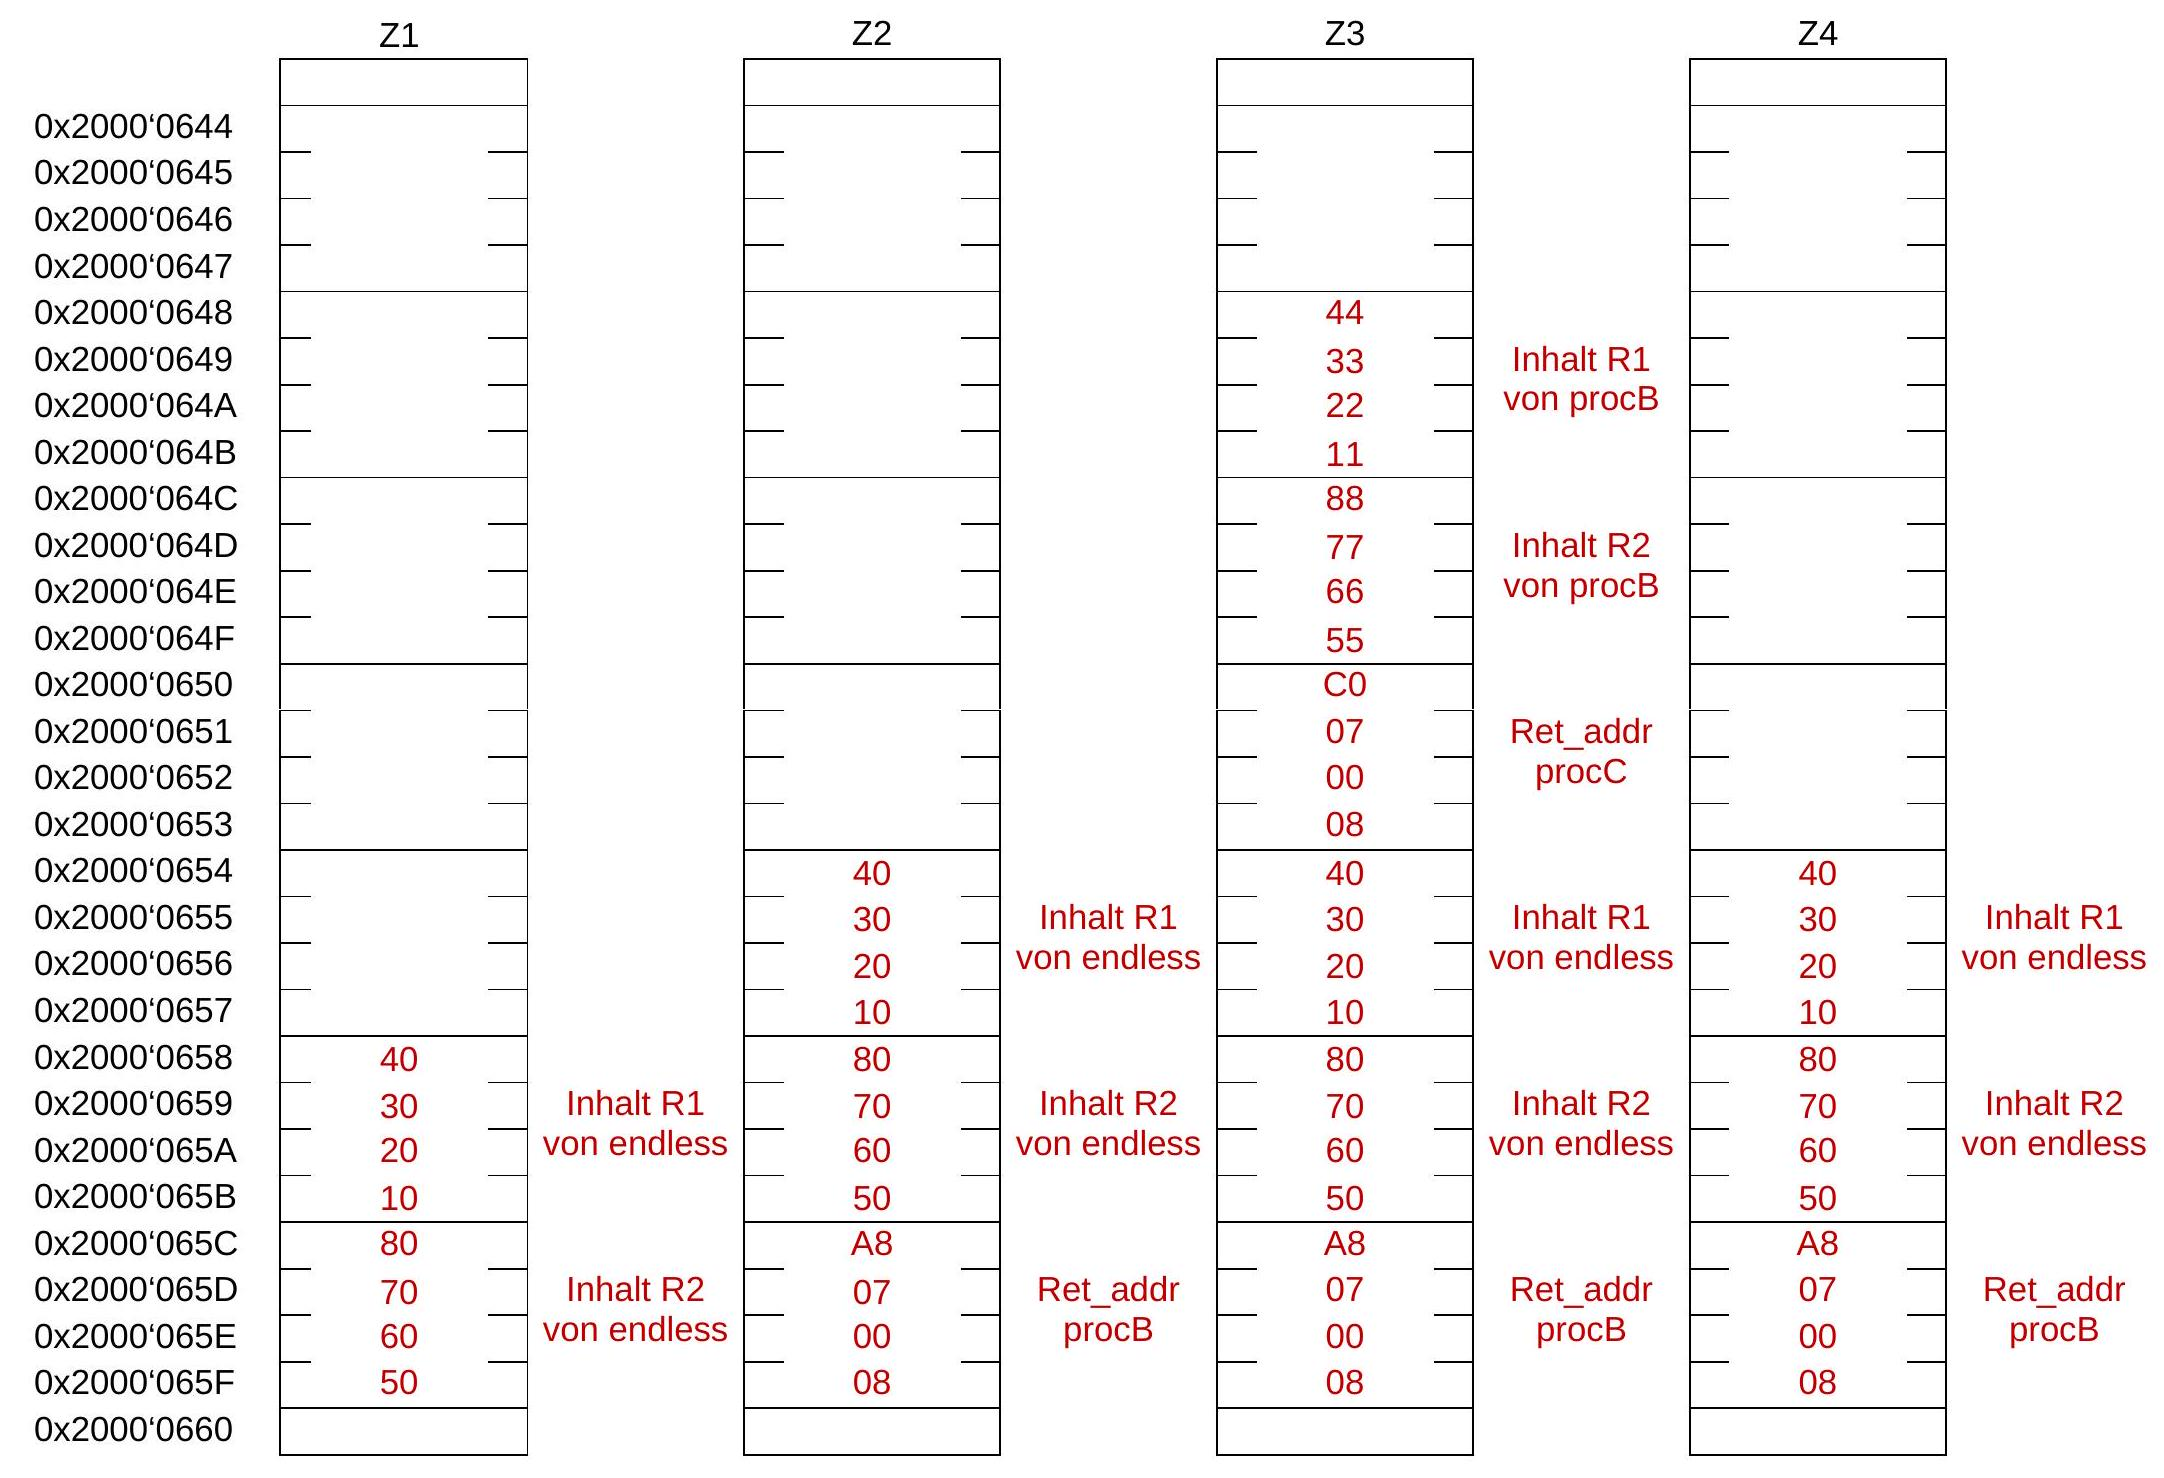
\includegraphics[width=\linewidth]{images/2025_01_02_88a231b00f1bec111bb0g-2}
\end{center}